\documentclass{article}
\usepackage{minted, graphicx, amsfonts, amssymb, amsmath, amsthm, float, subcaption} % Required for inserting images
\usepackage[english]{babel}
\usepackage[letterpaper,top=2cm,bottom=2cm,left=3cm,right=3cm,marginparwidth=1.75cm]{geometry}

\title{EE132 Lab 6}
\author{Andre Winkel, Russell Yang}
\date{\today}

\begin{document}
\maketitle

\begin{abstract}
    In this lab, we will explore underdamped second-order systems. We will analyze the damping ratio and natural frequency of our QUBE servo system in order to determine peak time and percent overshoot time-domain specifications. To do so, we will utilize the standard second-order transfer function, as well as the step response of the system.
\end{abstract}

\section{System built} 
\begin{figure} [H]
    \centering
    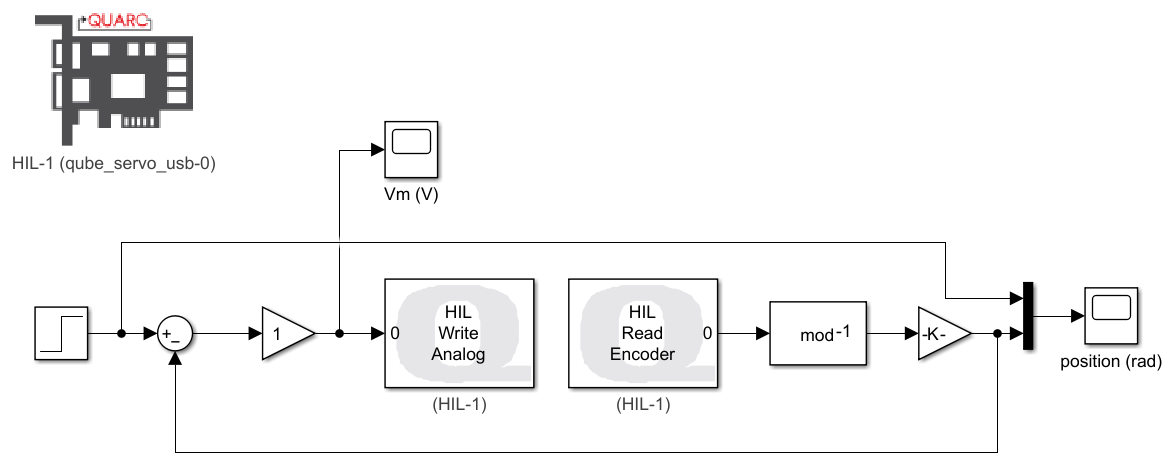
\includegraphics[width=0.75\linewidth]{system.png}
    \caption{Simulink model constructed for analysis}
    \label{fig:1}
\end{figure}

\section{In-Lab exercises and Results}
\subsection{Natural frequency and damping ratio of system}
Considering the standard second-order transfer function
\begin{equation}
    \frac{Y(s)}{R(s)}=\frac{\omega_n^2}{s^2+2\zeta\omega_ns+\omega^2_n},
\end{equation}
and the closed loop transfer function of the QUBE-Servo position control
\begin{equation}
    \frac{\Theta_d(s)}{V_m(s)}=\frac{\frac{K}{\tau}}{s^2+\frac{1}{\tau}s+\frac{K}{\tau}},
\end{equation}
we can determine the natural frequency and damping ratio of the system. Considering the steady state gain $K=23.0\frac{\text{rad}}{V_s}$ and the model time constant $\tau=0.13$s, we see that
\begin{equation} \notag
    \frac{\Theta_d(s)}{V_m(s)}=\frac{176.9}{s^2+7.692s+176.9}.
\end{equation}
Then,
\begin{equation} \notag
    \omega_n=\sqrt{176.9}=13.4
\end{equation}
and
\begin{equation} \notag
    \zeta=\frac{1}{\tau(2)(13.4)}=0.287.
\end{equation}

\subsection{Expected peak time and overshoot}
We then consider our equation for percent overshoot,
\begin{equation}
    PO=100e^{\left(-\frac{\pi\zeta}{\sqrt{1-\zeta^2}}\right)},
\end{equation}
and our equation for the peak time,
\begin{equation}
    t_p=\frac{\pi}{\omega_n\sqrt{1-\zeta^2}},
\end{equation}
we are able to determine
\begin{equation} \notag
    PO=39.014\%
\end{equation}
and
\begin{equation} \notag
    t_p=0.2447\text{s}.
\end{equation}

\subsection{System response}
Below, we observe the QUBE-Servo's response when we build and run the QUARC controller:
\begin{figure}[H]
    \centering
    \begin{subfigure}[b]{0.45\linewidth}
        \centering
        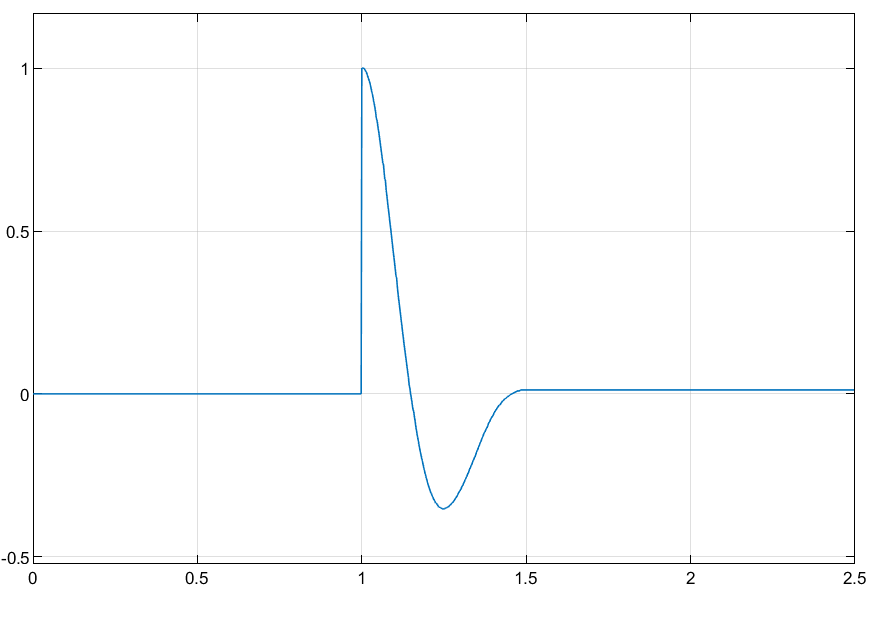
\includegraphics[width=\linewidth]{voltage.png}
        \caption{Voltage input}
        \label{fig:voltage}
    \end{subfigure}
    \hfill
    \begin{subfigure}[b]{0.45\linewidth}
        \centering
        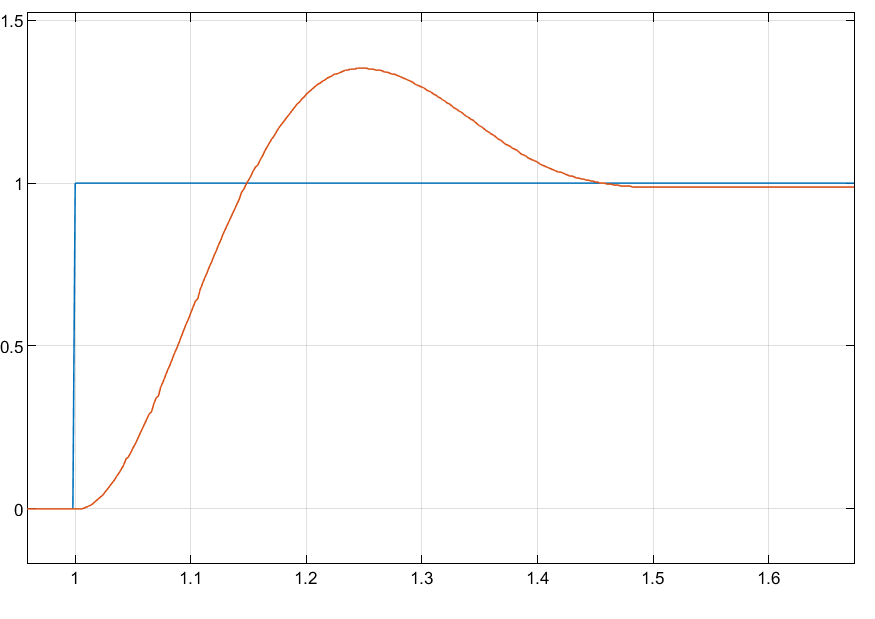
\includegraphics[width=\linewidth]{position.png}
        \caption{Load position}
        \label{fig:position}
    \end{subfigure}
    \caption{System response}
    \label{fig:response}
\end{figure}

\subsection{Measured peak time and percent overshoot}
\begin{figure} [H]
    \centering
    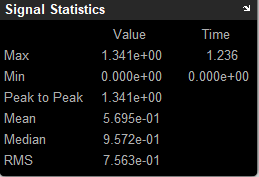
\includegraphics[width=0.5\linewidth]{measured.png}
    \caption{Signal statistics for position}
    \label{fig:statistics}
\end{figure}
From the plots and signal statistics tool, we can observe the peak time to be 1.235 seconds, and the maximum position to be 1.341 radians. Using these values as well as our percent overshoot equation,
\begin{equation}
    PO=\frac {100(y_{\text{max}}-R_0)}{R_0},
\end{equation}
we find our percent overshoot to be $34.1\%$. Considering the input begins at $1$s, our real peak time is $t_p=0.235$s.

\section{Analysis}
One of the primary issues we encountered in our calculation was our data collection, that is to say, saving data to Matlab for offline analysis. Instead, we used the built-in signal statistics menu which allowed us to observe the values that we cared about, our maximums. From here, we were able to determine the peak time and calculate the percent overshoot. Comparing the measured values to our derived values was rather straightforward, as the differences between them were fairly negligible. The largest difference we observed was in the percent overshoot, as our calculated value was $39.014\%$, and our measured value was $34.1\%$, which is still a fairly negligible difference. On the contrary, our measured $t_p=0.235$s, and our calculated $t_p=0.2447$s, which is an even more minute difference (no pun intended). Thus, we encountered no other issues in deriving or calculating our values for peak time and percent overshoot for this system.

\section{Conclusion}
In this lab, we were able to determine the theoretical natural frequency and damping ratio of the system, as well as determine the peak time and percent overshoot using these derived parameters. We then experimentally determined the peak time and percent overshoot using Simulink, and compared them to our theoretical values. We were then able to verify the accuracy of the model steady state gain and the time constant, as our measured values were very similar to our derived values.

\end{document}